\section{\green{Results}}

\subsection{\green{Training}}
Throughout the five epochs, each consisting of 2.000 E- and M-steps with a batch size of four, the model generated approximately 80.000 programs per task, training for about three days. During this phase, the model successfully solved 33 out of the 48 tasks it was trained on, representing a 50\% split.

As depicted in Figure \ref{fig:program_variations_binary_train}, an average of about 11.000 unique programs were created per task, indicating that approximately one-eighth of the programs were resampled, while the rest were distinct. This data also reveals certain task groups that posed more significant challenges than others. For instance, none of the tasks in the \texttt{caesar-cipher-k-modulo-n} group were solved, whereas all tasks in the \texttt{prepend-index-k} or \texttt{mult-k} groups were successfully completed. Refer to Tables \ref{tab:task_ex} and \ref{tab:task_programs} for examples and correct solutions, respectively.

\begin{figure}[H]
    \centering
    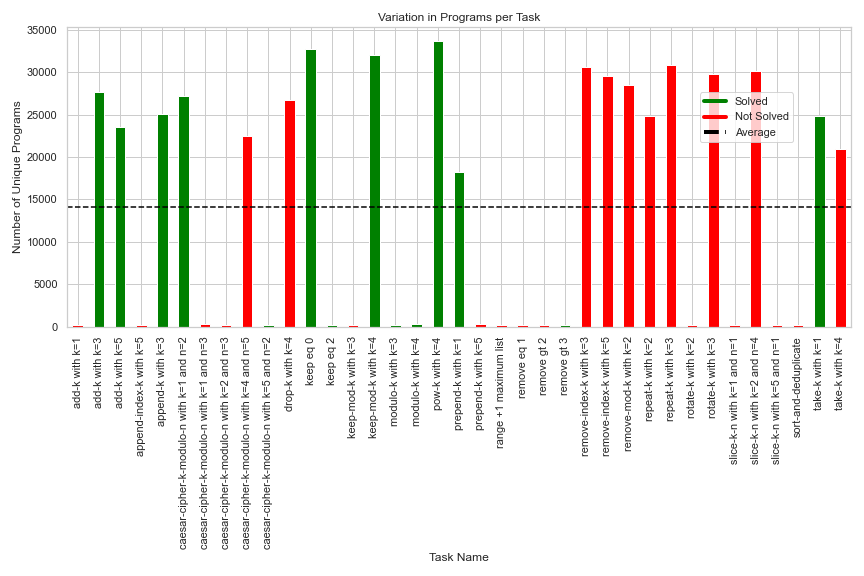
\includegraphics[width=\textwidth]{../img/plot_program_variations_binary_train.png}
    \caption{Bar plot of unique programs created per task. The sorted tasks the model has been trained are on the x-axis and the number of unique programs that have been created per task are on the y-axis. Bars of tasks that have been solved are coloured green and unsolved tasks are coloured red. The black dotted line demarcates the average number of uniquely created programs.}
    \label{fig:program_variations_binary_train}
\end{figure}


An examination of the model's improvement across consecutive Expectation-Maximization (E-M) cycles is shown in Figure \ref{fig:em_cycles}. The plot shows a clear upward trend in the average cumulative number of solutions, suggesting progressive improvement in both the forward policy and the generative model.

\begin{figure}[H]
    \centering
    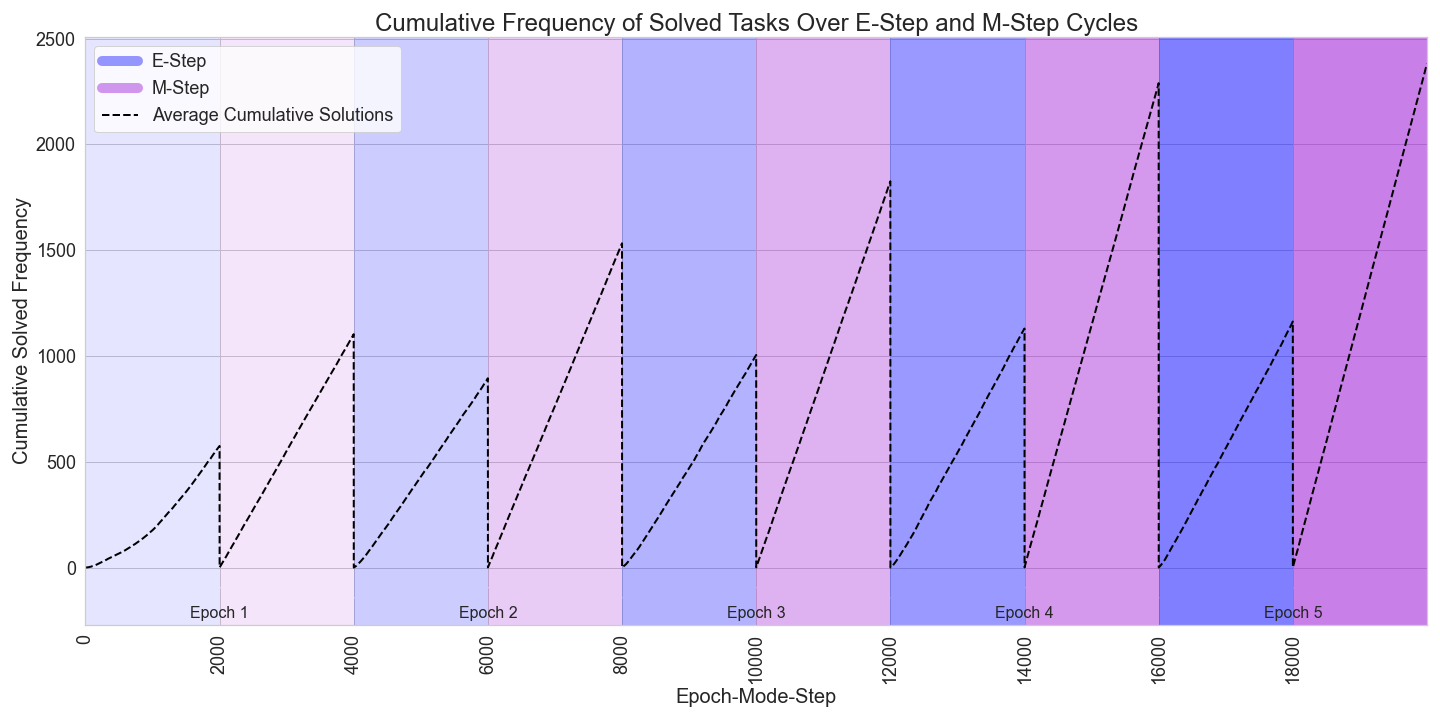
\includegraphics[width=\textwidth]{../img/em_cycles.png}
    \caption{The plot displays the cumulative number of tasks solved (y-axis) against the number of steps (x-axis). Each step represents an iteration in the E-M cycle. The initial 2.000 steps correspond to the first E-step, marked with a blue background, followed by the first M-step spanning the next 2.000 steps (up to step 4.000), distinguished by a purple background. This pattern constitutes one complete epoch. The graph includes a dotted line representing the average number of tasks solved over all epochs, offering a benchmark for comparison. Furthermore, the intensity of the color hue in the plot encodes the temporal sequence of the epochs: brighter bars on the left signify earlier epochs (the first epoch), with the hue gradually darkening towards the right, culminating in the fifth and final epoch.}
    \label{fig:em_cycles}
\end{figure}


\subsection{\green{Inference}}
During inference, the model attempted to solve all 95 tasks sequentially, producing 400 programs in about 100 steps, taking roughly 30 seconds for each task. FlowCoder solved 42 tasks.

Figure \ref{fig:program_variations_binary_inference} demonstrates the variance in task difficulty during inference. The \texttt{caesar} tasks often resulted in similar solutions, as seen from the limited diversity in program attempts, whereas a broader range of strategies was explored in other unsolved tasks. The solved tasks showed varying degrees of program exploration. On average, approximately 145 unique programs were generated per task.

\begin{figure}[H]
    \centering
    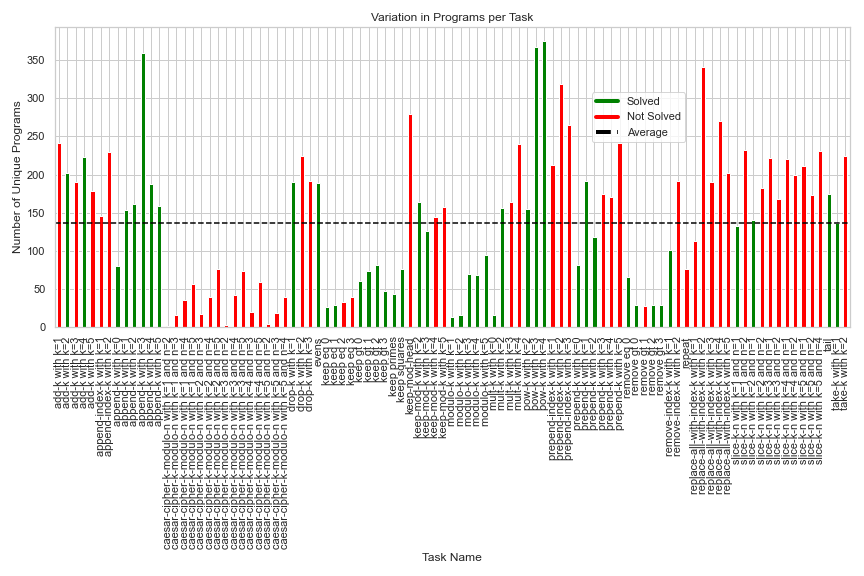
\includegraphics[width=\textwidth]{../img/plot_program_variations_binary_inference.png}
    \caption{Analysis of the number of unique programs generated per task during inference, as shown in Figure \ref{fig:program_variations_binary_inference}. Tasks are listed on the x-axis, and the count of unique programs is on the y-axis. The figure highlights the variance in program generation across tasks, with \texttt{caesar} tasks often showing limited program diversity, in contrast to other tasks that exhibit a wide range of attempts. The average number of unique programs created per task is approximately 145, indicating varied program attempts.}
    \label{fig:program_variations_binary_inference}
\end{figure}

\todo[inline]{maybe take this plot out?}

A key finding is that 13 tasks, unsolved and unseen during training, were successfully tackled in the inference phase, as shown in Figure \ref{fig:solution_variations_inference}. Notably, 11 of these tasks belong to groups where at least one task was solved during training, e.g. the model was trained (and solved) tasks \texttt{append-k} with \texttt{k=0, k=2, k=3} and during inference the model solved tasks \texttt{append-k} with \texttt{k=1, k=4, k=5}, which were previously unseen. Interestingly, 2 tasks were solved during inference without any precedent of tasks of a similar task group being seen in training. Additionally, it is observed that all tasks solved exclusively during inference had not been exposed to the model in the training phase.
The distribution of unique solutions also reveals that multiple tasks, irrespective of their exposure during training, exhibited a range of solutions. This diversity in solutions reflects the model's capacity to explore the solution space comprehensively, aligning with our goal of not merely finding a point estimate but understanding the entire posterior distribution of solutions for each task.

\begin{figure}[ht]
    \centering
    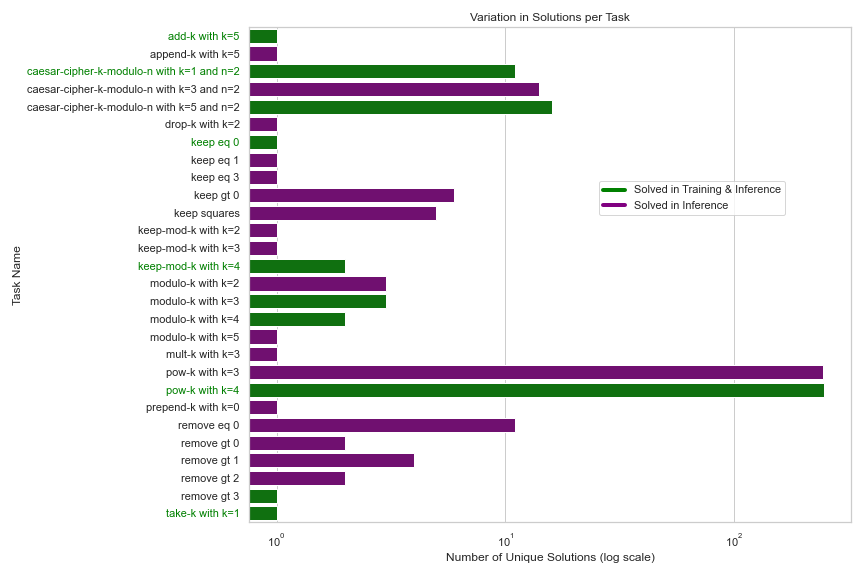
\includegraphics[width=\textwidth]{../img/plot_solution_variations_inference.png}
    \caption{Distribution of unique solutions per task during inference, displayed in a log-scaled bar chart. The y-axis lists the task names, while the x-axis quantifies the number of unique solutions. The chart reveals that 13 tasks not solved in training were resolved during inference, with 11 belonging to groups with at least one task previously solved in training. Only solved tasks are shown.}
    \label{fig:solution_variations_inference}
    \end{figure}

In table \ref{tab:multiple_solutions} we can see an example of varied solutions to a task. The model has found the shortest solution but also alternate solutions of the same task.

\begin{table}[H]
    \centering
    \begin{tabular}{|l|c|}
        \hline
        \textbf{Task} & \textbf{Solution}  \\\hline
        \texttt{append-k with k=2} & \texttt{(append 2 var0)} \\
        \texttt{} & \texttt{(append (mod 4 2) var0)} \\
        \texttt{} & \texttt{(append (min 4 2) var0)} \\
        \texttt{} & \texttt{(append (mod 5 2) var0)} \\
        \hline
    \end{tabular}
    \caption{Multiple found solutions.}
    \label{tab:multiple_solutions}
\end{table}

On average, FlowCoder efficiently solves a task within approximately 8 steps. Notably, as illustrated in Figure \ref{fig:plot_min_step_for_solution_inference}, around half of the tasks are successfully resolved on the initial attempt. The model is able to rapidly solve many tasks that it had not encountered previously, often requiring fewer steps than the average.

\begin{figure}[H]
    \centering
    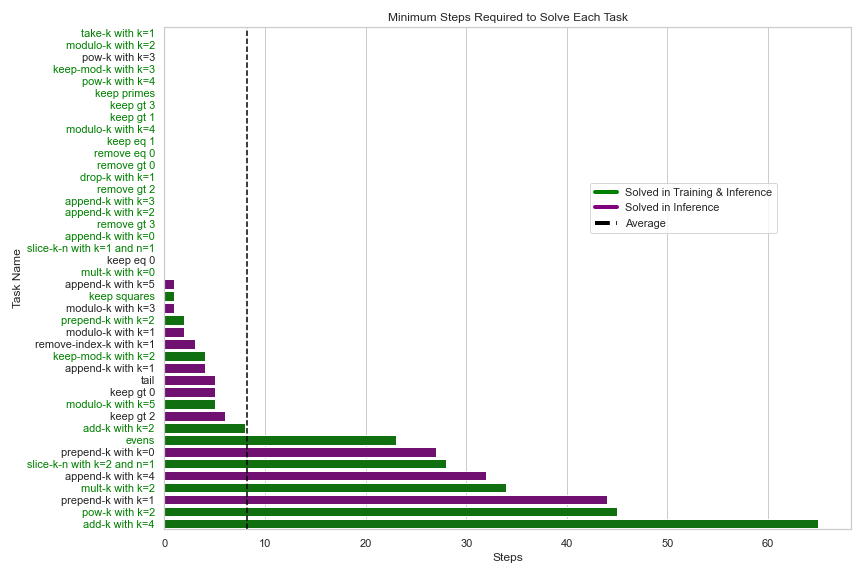
\includegraphics[width=\textwidth]{../img/plot_min_step_for_solution_inference.png}
    \caption{Analysis of the minimum number of steps required to solve tasks during inference. The x-axis represents the number of steps, and the y-axis lists the task names, sorted by the number of steps taken to find a solution. The dotted line indicates the average number of steps needed. Tasks solved both during training and inference are highlighted in green, whereas tasks exclusively solved during inference are in purple. Only solved tasks are shown.}
    \label{fig:plot_min_step_for_solution_inference}
\end{figure}
